\chapter{Phân tích và thiết kế}
\section{Phân tích}
\subsection{Business Process Modeling}
\begin{figure}[H]
    \centering
    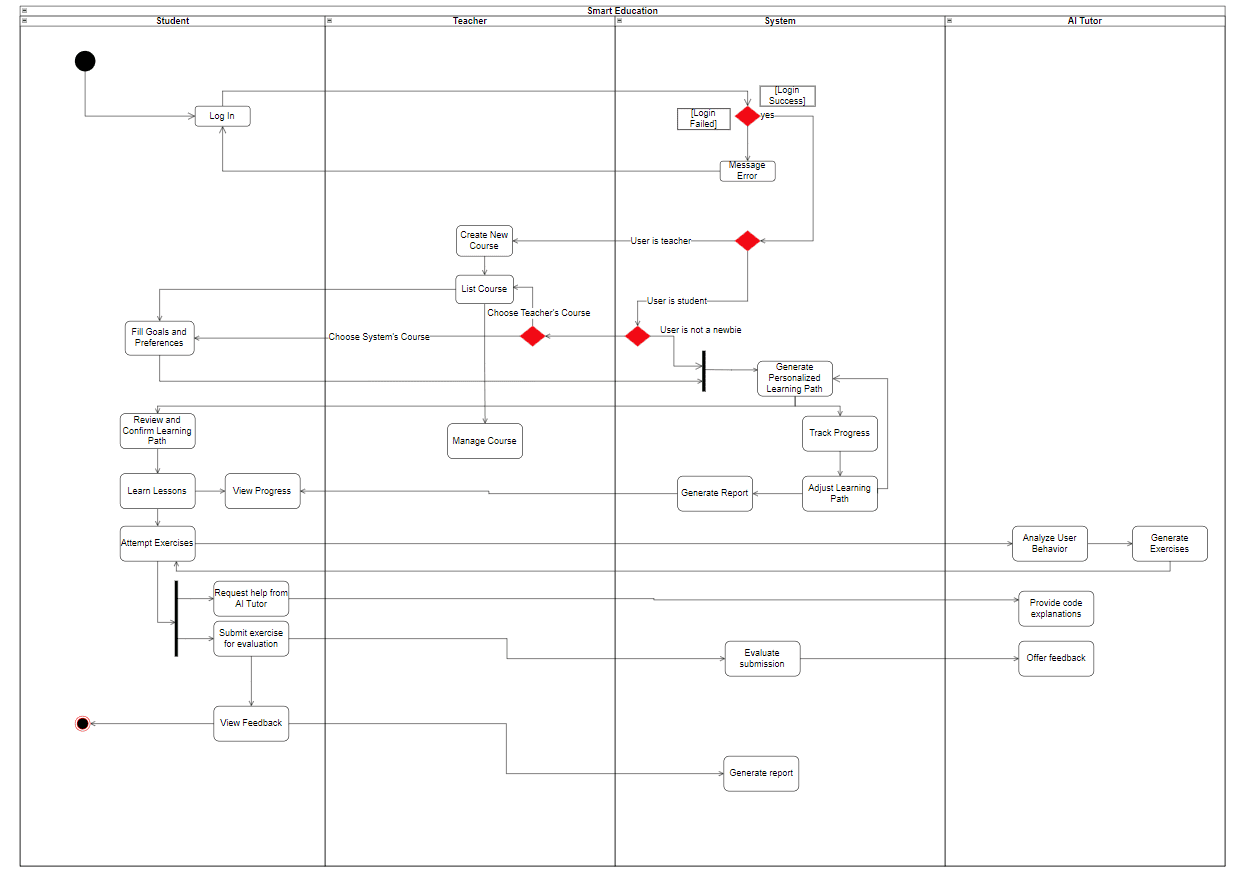
\includegraphics[width=\linewidth]{Images/Anh/activity.png}
    \caption{Activity diagram}
    \label{fig:enter-label}
\end{figure}
Activity diagram mô tả quy trình tương tác giữa bốn Actors: \textbf{\textit{Student (Học sinh), Teacher (Giáo viên), System (Hệ thống), và AI Tutor (Gia sư AI)}} trong hệ thống giáo dục thông minh. \par Học sinh bắt đầu bằng việc đăng nhập và tùy thuộc vào vai trò của họ (giáo viên hoặc học sinh), các hành động khác nhau sẽ diễn ra. Giáo viên có thể tạo khóa học mới hoặc chọn khóa học hiện có để quản lý, trong khi học sinh sẽ xác định mục tiêu học tập và xác nhận lộ trình học do hệ thống đề xuất. Sau đó, học sinh có thể học bài, thực hiện bài tập, và nếu cần có thể yêu cầu trợ giúp từ AI Tutor. Hệ thống cũng tự động theo dõi tiến độ học tập, điều chỉnh lộ trình và đánh giá bài nộp của học sinh. AI Tutor hỗ trợ bằng cách phân tích hành vi, giải thích mã code, và tạo bài tập phù hợp.
\subsection{Use case diagrams}
\begin{figure}[H]
    \centering
    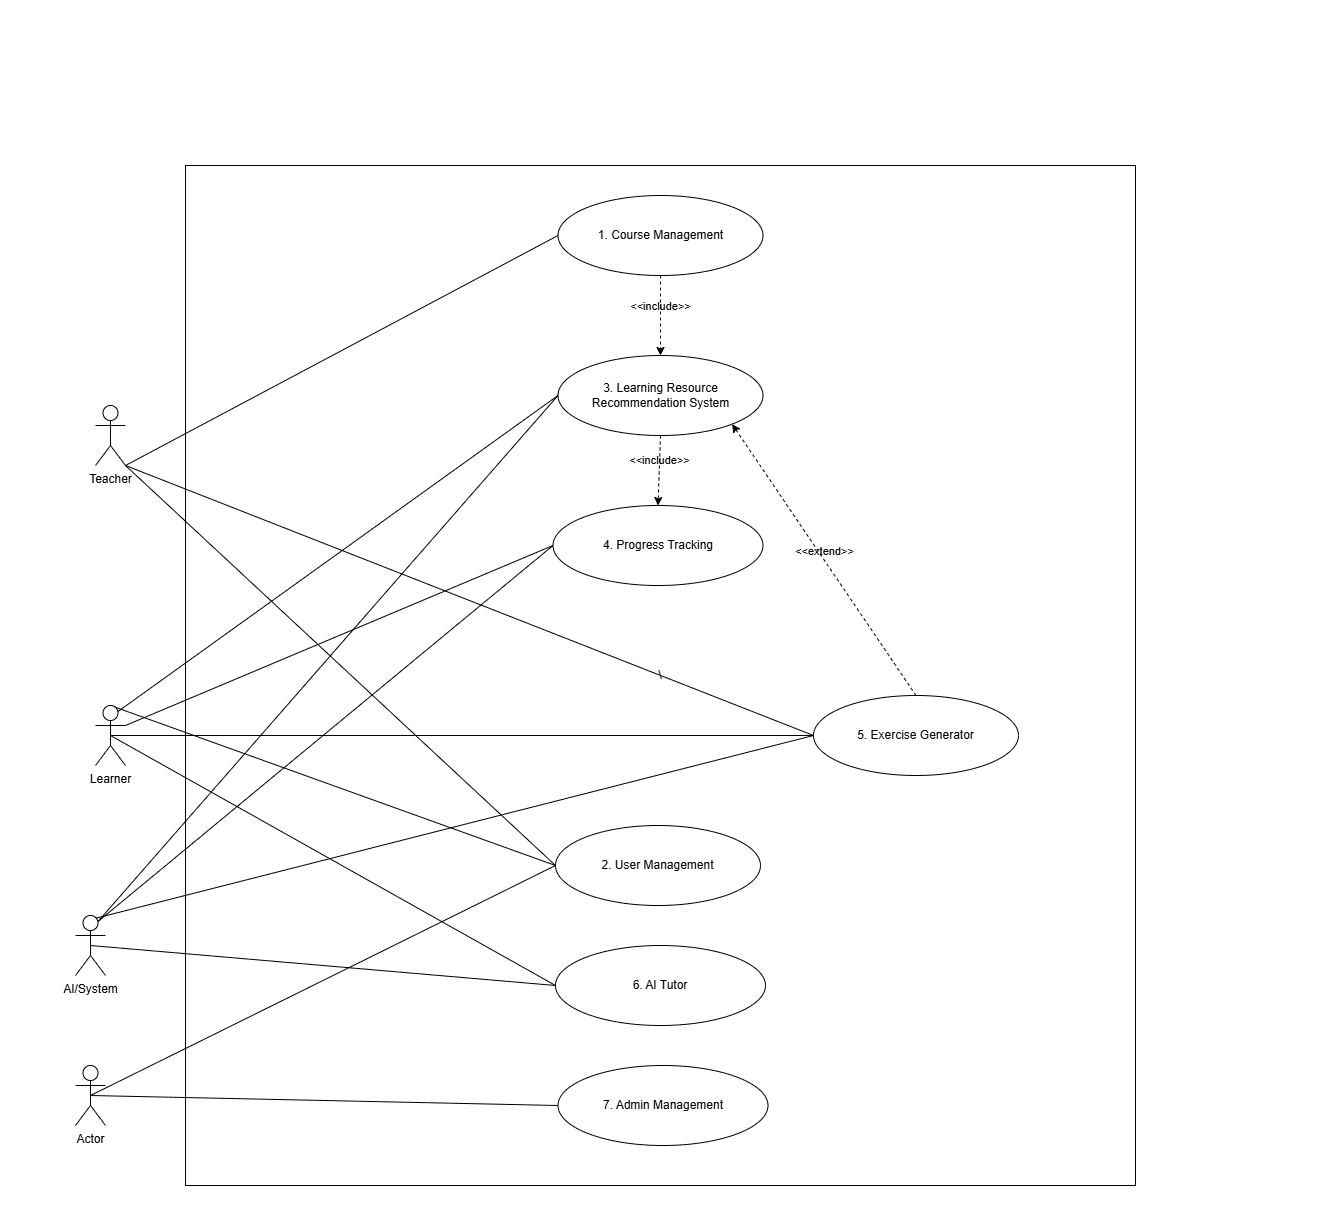
\includegraphics[scale=0.3]{Images/Usecase/usecase-All.drawio.png}
    \caption{Use case diagram}
    \label{fig:enter-label}
\end{figure}
\quad Mô hình use case tổng thể cho hệ thống học tập thông minh bao gồm ba tác nhân chính: Giáo viên, Người học, Quản trị viên và Hệ thống/AI. Các use case bao gồm Quản lý khóa học, Quản lý người dùng, Quản lý lộ trình học tập thích ứng, Theo dõi tiến độ, Tạo bài tập, Quản lý hệ thống cho Quản trị viên và Gia sư AI.
\subsubsection{Course Management}
\begin{figure}[H]
    \centering
    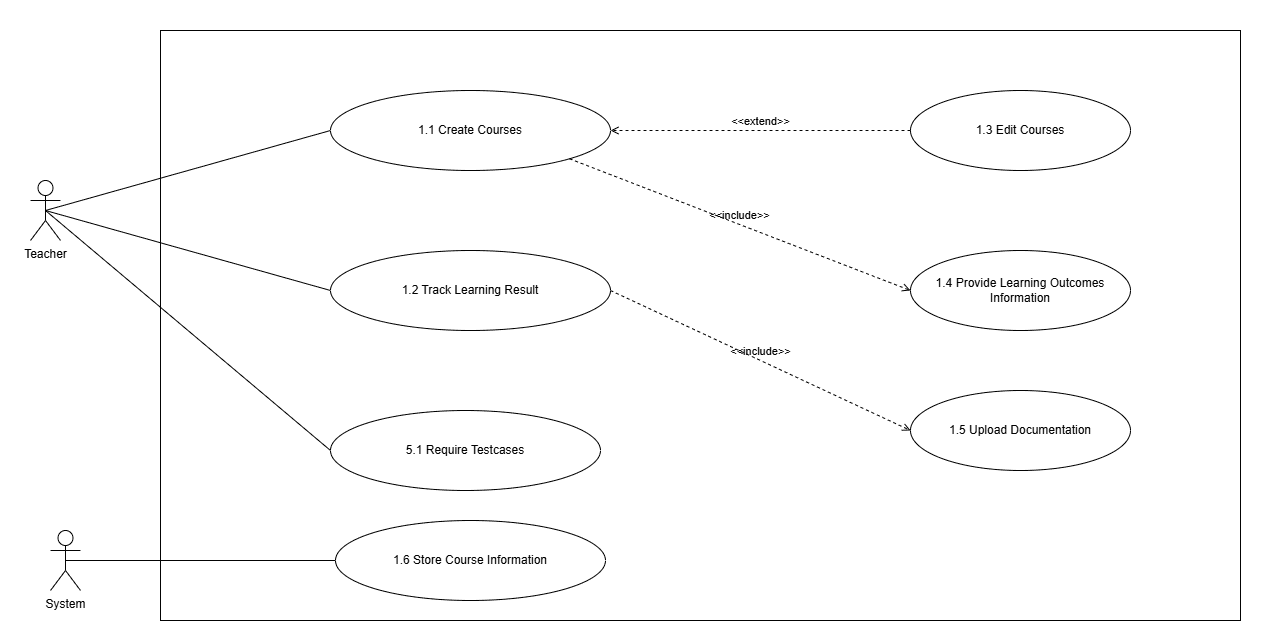
\includegraphics[scale=0.4]{Images/Usecase/usecase-Course Management.drawio.png}
    \caption{Detailed use case with id 1: Course Management}
    \label{fig:enter-label}
\end{figure}
\quad Use case \textbf{\textit{Quản lý khóa học}} bao gồm ba chức năng chính: Tạo khóa học, Theo dõi kết quả học tập và Yêu cầu bài kiểm tra. Use case  \textbf{\textit{"Chỉnh sửa khóa học"}} được mở rộng từ  \textbf{\textit{"Tạo khóa học"}}, cho thấy việc chỉnh sửa là một phần mở rộng tùy chọn của quá trình tạo khóa học. Use case diagram thể hiện các trách nhiệm chính của giáo viên trong việc quản lý khóa học trong hệ thống.
\par Ngoài ra, ở module này, Hệ thống sẽ có nhiệm vụ lưu trữ thông tin về khóa học mà giáo viên đã tạo ra. 
\subsubsection{User Management}
\begin{figure}[H]
    \centering
    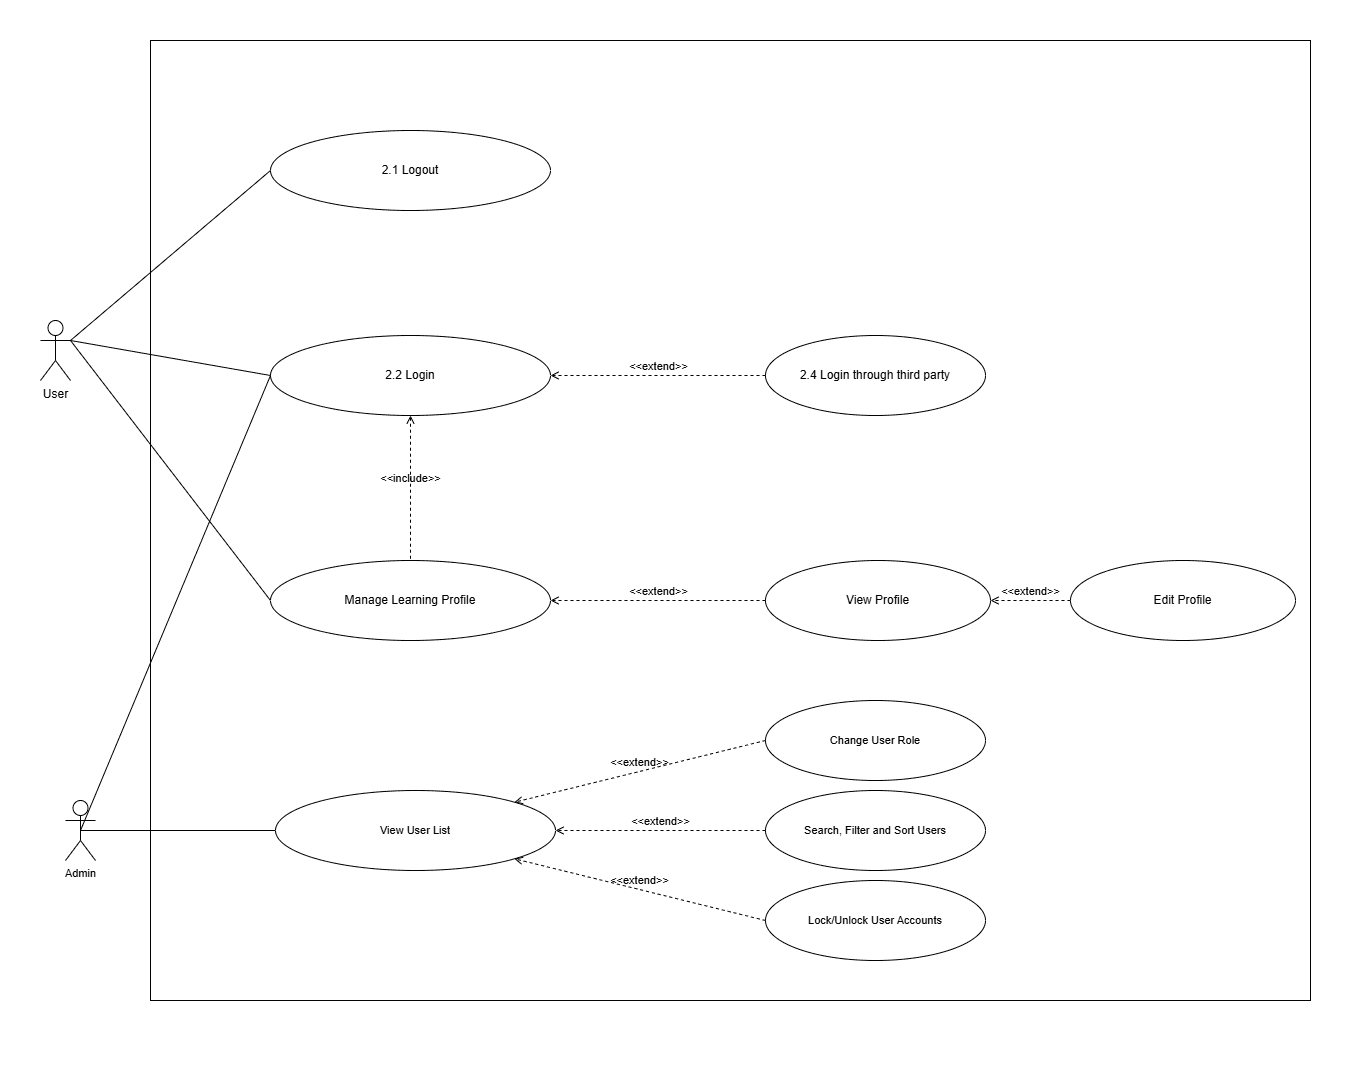
\includegraphics[scale=0.4]{Images/Usecase/usecase-User Management.drawio.png}
    \caption{Detailed use case with id 2: User Management}
    \label{fig:enter-label}
\end{figure}
\quad Use case  \textbf{\textit{Quản lý người dùng}}, tập trung vào tác nhân Người dùng bao gồm các chức năng như Đăng nhập, Đăng xuất, Quản lý hồ sơ học tập và Xem hồ sơ. Use case diagram cho thấy  \textbf{\textit{"Đăng nhập qua third-party"}} mở rộng từ use case  \textbf{\textit{"Đăng nhập"}} cơ bản, cung cấp một phương thức đăng nhập thay thế. Ngoài ra,  \textbf{\textit{"Xem hồ sơ"}} được thể hiện như một phần mở rộng của  \textbf{\textit{"Quản lý hồ sơ học tập"}}, cho thấy đây là một hành động liên quan nhưng riêng biệt. \par Quản trị viên có quyền đăng nhập bằng tài khoản của mình, từ đó \textbf{\textit{"Xem danh sách người dùng"}} sử dụng hệ thống. Ngoài ra, quản trị viên có thể \textbf{\textit{"Tìm kiếm, Lọc và Sắp xếp theo thông tin người dùng"}}, \textbf{\textit{"Vô hiệu hóa tài khoản/Kích hoạt tài khoản"}} và \textbf{\textit{" Thay đổi quyền truy cập của người dùng"}}. Ví dụ: Thay đổi từ người học sang giảng viên. 
\subsubsection{Learning Resource Recommendation System}
\begin{figure}[H]
    \centering
    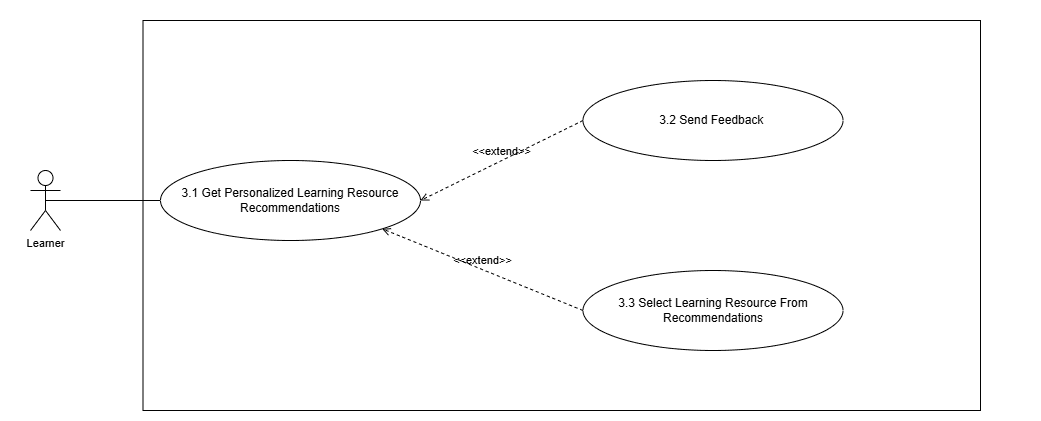
\includegraphics[scale=0.45]{Images/Usecase/usecase-Learning Resource Recommendation System - Learner.drawio.png}
    \caption{Detailed use case with id 3: Adaptive Learning Path Management of Learner Actor}
    \label{fig:enter-label}
\end{figure}
\quad Tác nhân chính trong biểu đồ trên là người học (Learner), có thể tương tác với hệ thống để nhận các đề xuất tài nguyên học tập. Use case \textbf{\textit{"Get Personalized Learning Resource Recommendations"}} cung cấp cho người học các tài nguyên học tập phù hợp với nhu cầu và lịch sử học tập của họ. Use case \textbf{\textit{"Send Feedback"}} có mối quan hệ \textbf{\textit{"<extend>"}} với \textbf{\textit{"Get Personalized Learning Resource Recommendations"}}, vì người học có thể gửi phản hồi về các tài nguyên đã được đề xuất để cải thiện hệ thống.
Use case \textbf{\textit{"Select Learning Resource From Recommendations"}} cũng mở rộng từ \textbf{\textit{"Get Personalized Learning Resource Recommendations"}}, cho phép người học tự chọn các tài nguyên mà họ thấy phù hợp với mục tiêu cá nhân.
\begin{figure}[H]
    \centering
    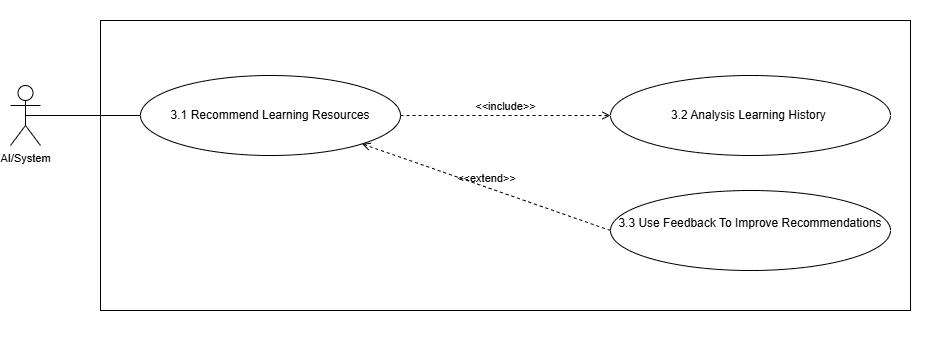
\includegraphics[scale=0.45]{Images/Usecase/usecase-Learning Resource Recommendation System - System.drawio.png}
    \caption{Detailed use case with id 3: Learning Resource Recommendation System of System Actor}
    \label{fig:enter-label}
\end{figure}
\quad Tác nhân chính là hệ thống AI, có nhiệm vụ chính là đề xuất tài nguyên học tập cá nhân hóa cho người dùng. Use case \textbf{\textit{"Recommend Learning Resources"}} bao gồm hoạt động \textbf{\textit{"Analysis Learning History"}} (phân tích lịch sử học tập), do quá trình phân tích lịch sử học tập là một phần không thể thiếu khi hệ thống tạo ra các đề xuất. Hệ thống có thể mở rộng thêm use case \textbf{\textit{"Use Feedback To Improve Recommendations"}} (sử dụng phản hồi để cải thiện đề xuất) dựa trên các phản hồi người dùng, giúp tinh chỉnh và nâng cao chất lượng đề xuất. Mối quan hệ \textbf{\textit{"<include>"}} được sử dụng giữa \textbf{\textit{"Recommend Learning Resources"}} và \textbf{\textit{"Analysis Learning History"}} vì quá trình phân tích là cần thiết. Mối quan hệ \textbf{\textit{"<extend>"}} giữa \textbf{\textit{"Recommend Learning Resources"}} và \textbf{\textit{"Use Feedback To Improve Recommendations"}} vì cải thiện đề xuất dựa trên phản hồi là một phần mở rộng có thể xảy ra tùy theo ngữ cảnh.

\subsubsection{Progress Tracking}
\begin{figure}[H]
    \centering
    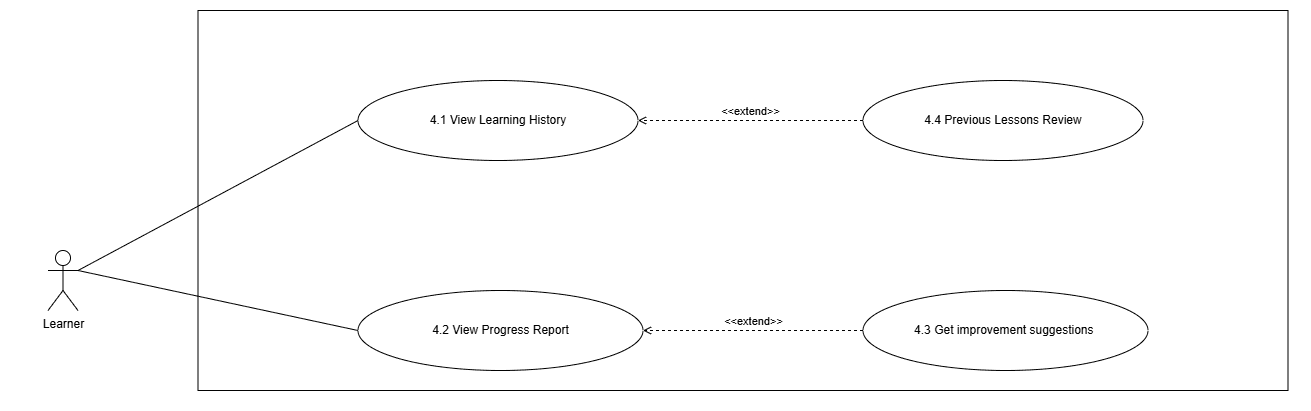
\includegraphics[scale=0.35]{Images/Usecase/usecase-Progress Tracking - Learner.drawio.png}
    \caption{Detailed use case with id 4: Progress Tracking of Learner Actor}
    \label{fig:enter-label}
\end{figure}
\quad Use case diagram trên thể hiện các chức năng  \textbf{\textit{Theo dõi tiến độ dành cho Người học}}. Có hai use case chính là  \textbf{\textit{"Xem lịch sử học tập"}} và  \textbf{\textit{"Xem báo cáo tiến độ"}}.  \textbf{\textit{"Xem lịch sử học tập"}} mở rộng đến  \textbf{\textit{"Xem lại các bài học trước đó"}}, cho phép người học ôn tập.  \textbf{\textit{"Xem báo cáo tiến độ"}} mở rộng đến  \textbf{\textit{"Nhận đề xuất cải thiện"}}, cung cấp hướng dẫn cá nhân hóa, nhấn mạnh việc theo dõi và phản hồi liên tục để hỗ trợ quá trình học tập của người dùng.
\begin{figure}[H]
    \centering
    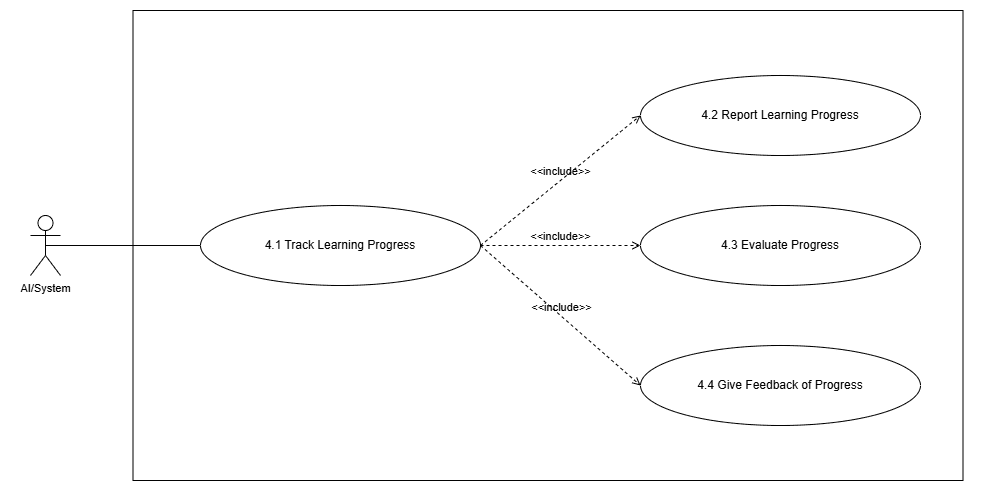
\includegraphics[scale=0.4]{Images/Usecase/usecase-Progress Tracking - System.drawio.png}
    \caption{Detailed use case with id 4: Progress Tracking of System Actor}
    \label{fig:enter-label}
\end{figure}
\quad Sơ đồ use case của hệ thống \textbf{\textit{Exercise Generator}} mô tả các tương tác giữa người dùng và hệ thống. Người học có thể yêu cầu hệ thống tạo tự động các bài tập thông qua chức năng \textbf{\textit{"Request Auto Exercise Generation"}}, và sau đó thực hiện các bài tập đó để cải thiện kỹ năng của mình thông qua \textbf{\textit{"Do Exercise"}}. Bên cạnh đó, giảng viên có thể sử dụng chức năng \textbf{\textit{"Upload Exercise"}} để tải lên các đề bài hoặc bài tập, từ đó hệ thống sẽ tự động xử lý và tạo ra các test case nhằm kiểm tra độ chính xác của bài giải thông qua \textbf{\textit{"Generate Test Cases"}}. Sau khi các test case được tạo, giảng viên có thể sử dụng chức năng \textbf{\textit{"Review Test Cases"}} để xem xét và đánh giá các test case nhằm đảm bảo chúng phù hợp với nội dung bài tập và đáp ứng được yêu cầu giảng dạy. Các chức năng này giúp hệ thống tạo ra môi trường học tập linh hoạt, hỗ trợ hiệu quả cho người học và giảng viên.
\subsubsection{Exercise Generator}
\begin{figure}[H]
    \centering
    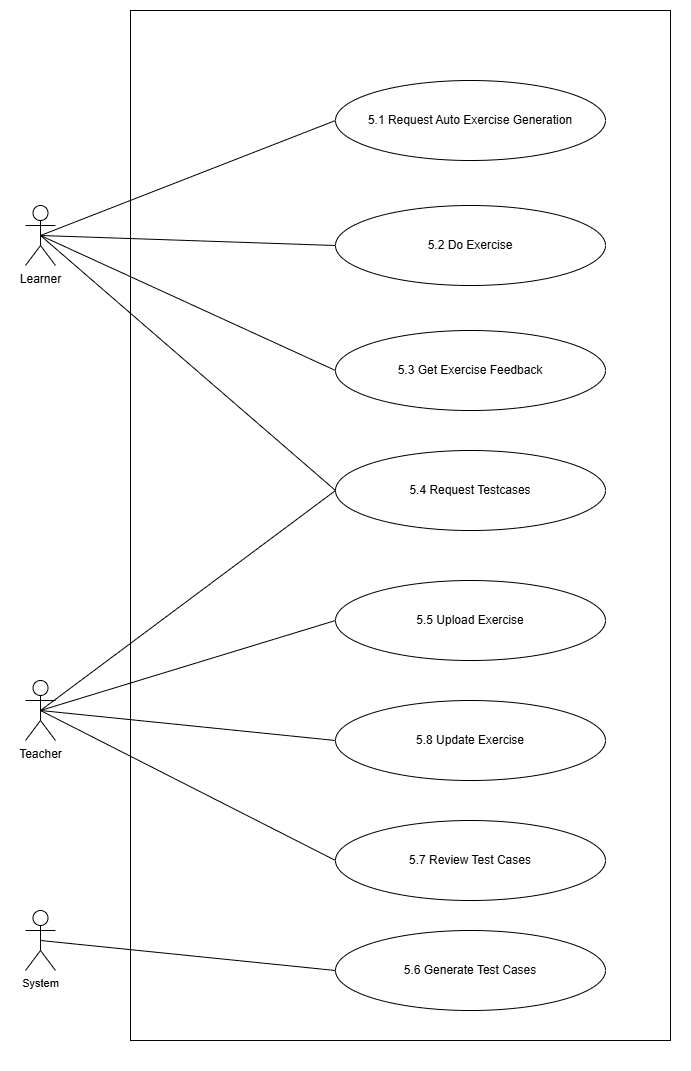
\includegraphics[scale=0.45]{Images/Usecase/usecase-Exercise Generator - Learner.drawio.png}
    \caption{Detailed use case with id 5: Exercise Generator}
    \label{fig:enter-label}
\end{figure}
\quad Use case diagram thể hiện các chức năng liên quan đến bài tập dành cho Người học. Có bốn use case chính:  \textbf{\textit{"Yêu cầu tạo bài tập tự động", "Làm bài tập", "Nhận phản hồi về bài tập", và "Yêu cầu bài kiểm tra"}}. Người học có thể yêu cầu hệ thống tạo bài tập tự động phù hợp với trình độ của họ. Sau khi làm bài tập, người học có thể nhận phản hồi để hiểu rõ hơn về kết quả của mình. Khả năng yêu cầu bài kiểm tra cho phép người học tự đánh giá kiến thức của mình khi cần.
\subsubsection{AI Tutor}
\begin{figure}[H]
    \centering
    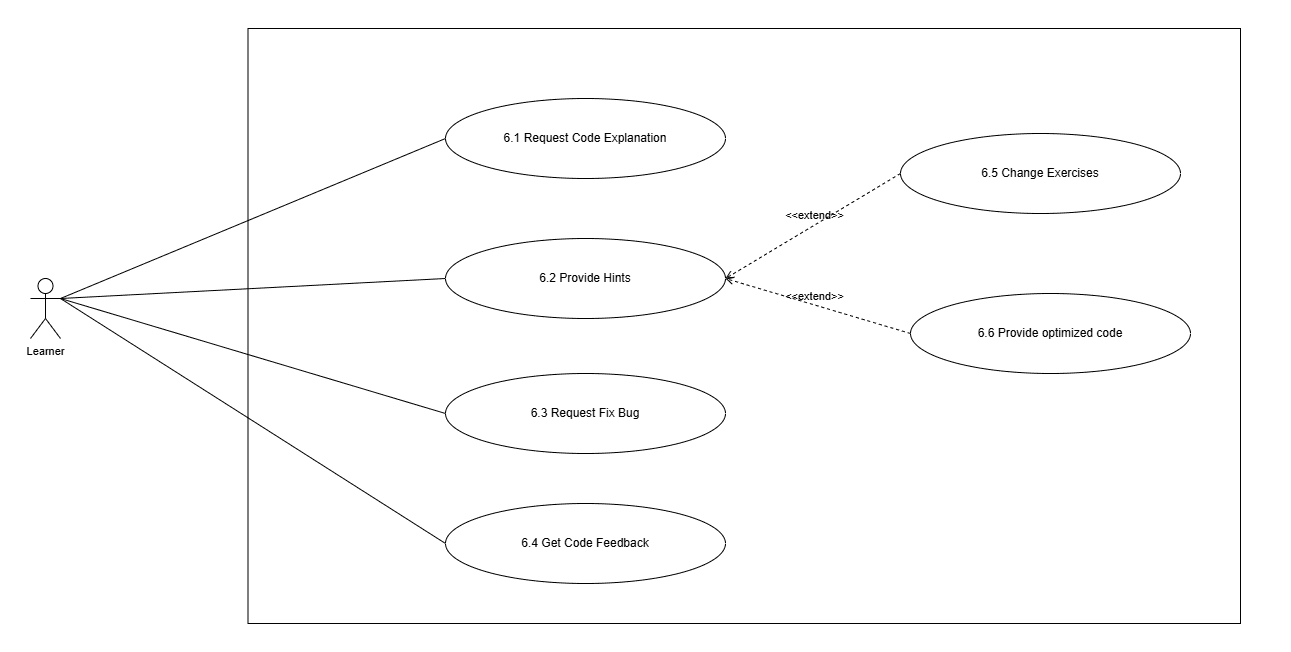
\includegraphics[scale=0.3]{Images/Usecase/usecase-AI Tutor - Learner.drawio.png}
    \caption{Detailed use case with id 6: AI Tutor of Learner Actor}
    \label{fig:enter-label}
\end{figure}
\quad Use case diagram thể hiện các chức năng của Gia sư AI dành cho Người học. Có bốn use case chính:  \textbf{\textit{"Yêu cầu giải thích mã", "Yêu cầu gợi ý", "Yêu cầu sửa lỗi", và "Nhận phản hồi về mã".}}
Người học có thể yêu cầu giải thích về mã nguồn để hiểu rõ hơn về cấu trúc và logic của code. Chức năng yêu cầu gợi ý có hai chức năng quan hệ \textbf{\textit{"extend"}} là \textbf{\textit{"Hỗ trợ chuyển đổi bài tập"}} dựa trên nhu cầu, học lực của người dùng và \textbf{\textit{"Cung cấp mã tối ưu hóa"}} giúp người học vượt qua các khó khăn trong quá trình học lập trình cũng như cải thiện tối đa kỹ thuật code của người dùng. Việc nhận phản hồi về mã giúp người học cải thiện kỹ năng lập trình của mình một cách liên tục.
\begin{figure}[H]
    \centering
    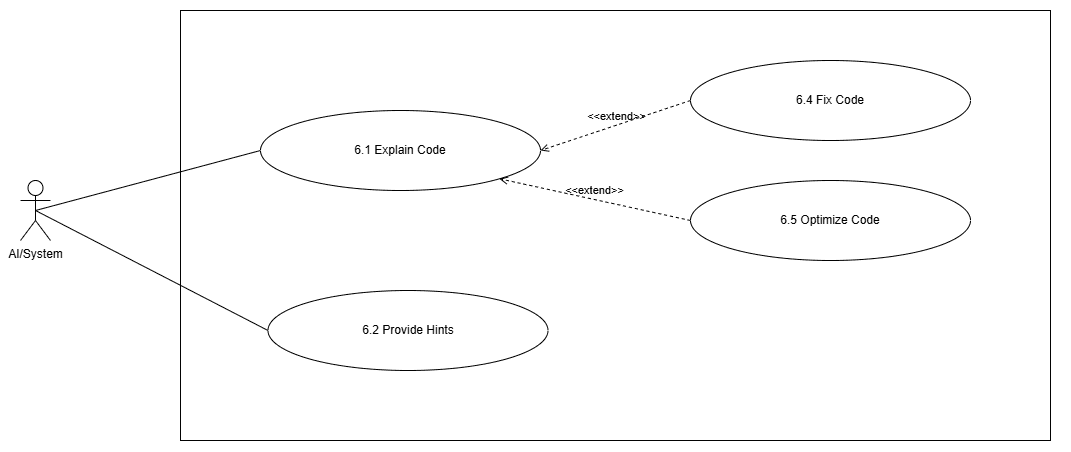
\includegraphics[scale=0.4]{Images/Usecase/usecase-AI Tutor - System.drawio.png}
    \caption{Detailed use case with id 6: AI Tutor of System Actor}
    \label{fig:enter-label}
\end{figure}
\quad Use case diagram trên mô tả  \textbf{\textit{hệ thống AI Tutor}} với vai trò hỗ trợ người dùng trong việc xử lý và hiểu mã lập trình. Hệ thống có khả năng  \textbf{\textit{giải thích mã lệnh (Use case 6.1)}} và  \textbf{\textit{cung cấp gợi ý khi người dùng gặp khó khăn (Use case 6.2)}}. Từ chức năng giải thích mã, hệ thống có thể mở rộng thêm các chức năng khác như  \textbf{\textit{sửa lỗi (Use case 6.4)}} và  \textbf{\textit{tối ưu mã lệnh (Use case 6.5)}}. Hệ thống nhằm mục tiêu hỗ trợ người dùng học lập trình hiệu quả hơn thông qua các công cụ hỗ trợ trực tiếp từ AI.
\newpage
\section{Thiết kế}
\subsection{Kiến trúc hệ thống}
\subsubsection{Phân tích kiến trúc hệ thống phổ biến hiện nay}
Hiện nay, có nhiều kiến trúc phần mềm khác nhau, mỗi loại có ưu và nhược điểm riêng, phù hợp với các loại dự án và yêu cầu cụ thể. Dưới đây là một số kiến trúc phần mềm phổ biến và các điểm chính của chúng:
\begin{enumerate}
    \item Kiến trúc Monolithic
    \begin{itemize}
        \item \textbf{\textit{Định nghĩa:}} Kiến trúc monolithic là một mô hình truyền thống trong đó toàn bộ ứng dụng được xây dựng như một đơn vị duy nhất, tích hợp chặt chẽ.
        \item \textbf{\textit{Điểm chính:}} 
        \begin{itemize}
            \item Đơn giản để phát triển, triển khai và kiểm thử
            \item Hiệu suất tốt do không có overhead của network calls
            \item Khó mở rộng và bảo trì khi ứng dụng phức tạp
            \item Khó áp dụng công nghệ mới cho từng phần của ứng dụng
        \end{itemize}
        \item \textbf{\textit{Ví dụ:}} Một ứng dụng web PHP truyền thống, nơi tất cả chức năng (UI, business logic, data access) đều nằm trong cùng một codebase.
    \end{itemize}
    \item Kiến trúc Microservices
    \begin{itemize}
        \item \textbf{\textit{Định nghĩa:}} Kiến trúc microservices chia nhỏ ứng dụng thành các dịch vụ độc lập, mỗi dịch vụ chịu trách nhiệm cho một chức năng cụ thể và có thể được phát triển, triển khai độc lập.
        \item \textbf{\textit{Điểm chính:}} 
        \begin{itemize}
            \item Dễ dàng mở rộng và bảo trì từng service riêng biệt
            \item Cho phép sử dụng công nghệ phù hợp nhất cho mỗi service
            \item Tăng cường khả năng chịu lỗi của hệ thống
            \item Phức tạp hơn trong việc quản lý và điều phối các service
        \end{itemize}
        \item \textbf{\textit{Ví dụ:}} Netflix sử dụng kiến trúc microservices, với các service riêng biệt cho việc xử lý video, quản lý người dùng, đề xuất nội dung, v.v.
    \end{itemize}
    \item Kiến trúc Client-Server
    \begin{itemize}
        \item \textbf{\textit{Định nghĩa:}} Kiến trúc client-server chia ứng dụng thành hai phần chính: client (trình bày và tương tác người dùng) và server (xử lý logic nghiệp vụ và lưu trữ dữ liệu).
        \item \textbf{\textit{Điểm chính:}} 
        \begin{itemize}
            \item Phân tách rõ ràng giữa client và server
            \item Dễ dàng mở rộng server để đáp ứng nhu cầu người dùng
            \item Cải thiện bảo mật thông qua kiểm soát truy cập tại server
            \item Phụ thuộc vào kết nối mạng giữa client và server
        \end{itemize}
        \item \textbf{\textit{Ví dụ:}} Một ứng dụng web với frontend (React) và backend (Node.js) giao tiếp qua RESTful API.
    \end{itemize}
    \item Kiến trúc Event-Driven
    \begin{itemize}
        \item \textbf{\textit{Định nghĩa:}} Kiến trúc event-driven là một mô hình trong đó việc tạo ra, phát hiện, tiêu thụ và phản ứng với các sự kiện là cốt lõi của hệ thống.
        \item \textbf{\textit{Điểm chính:}} 
        \begin{itemize}
            \item Tách rời các thành phần hệ thống, giảm sự phụ thuộc trực tiếp
            \item Khả năng mở rộng và linh hoạt cao
            \item Dễ dàng thêm chức năng mới mà không ảnh hưởng đến các thành phần hiện có
            \item Có thể phức tạp trong việc theo dõi luồng xử lý và debug
        \end{itemize}
        \item \textbf{\textit{Ví dụ:}} Hệ thống thương mại điện tử, khi một đơn hàng được đặt, một sự kiện "OrderPlaced" được phát ra, kích hoạt các quy trình xử lý khác như cập nhật kho, gửi email xác nhận, v.v.
    \end{itemize}
    \item Kiến trúc Serverless
    \begin{itemize}
        \item \textbf{\textit{Định nghĩa:}} Kiến trúc serverless cho phép phát triển và chạy ứng dụng mà không cần quản lý trực tiếp máy chủ, tập trung vào việc viết code cho các chức năng (functions) cụ thể.
        \item \textbf{\textit{Điểm chính:}} 
        \begin{itemize}
            \item Giảm chi phí vận hành và bảo trì hạ tầng
            \item Tự động mở rộng theo nhu cầu sử dụng
            \item Chỉ trả tiền cho tài nguyên thực sự sử dụng
            \item Có thể gặp vấn đề về cold start và vendor lock-in
        \end{itemize}
        \item \textbf{\textit{Ví dụ:}} Một ứng dụng xử lý ảnh sử dụng AWS Lambda để thực hiện các tác vụ như resize, filter, và lưu trữ ảnh khi người dùng tải lên.
    \end{itemize}
\end{enumerate}

\subsubsection{Lựa chọn kiến trúc hệ thống}
Dựa trên yêu cầu của hệ thống, nhóm quyết định sử dụng kiến trúc Client-Server. Cụ thể như sau:
\begin{enumerate}
    \item Client Tier:
    \begin{itemize}
        \item \textbf{Frontend:} Ứng dụng Vue.js cung cấp giao diện người dùng cho sinh viên, giảng viên và admin.
        \item \textbf{Chức năng:} Hiển thị nội dung học tập, quản lý khóa học, bài tập, lộ trình học tập và tương tác với người dùng.
        \item \textbf{Tương tác:} Giao tiếp với server thông qua RESTful API.
    \end{itemize}
    \item Server Tier:
    \begin{enumerate}
        \item \textbf{API Layer:}
        \begin{itemize}
            \item \textbf{Framework:} FastAPI xử lý các yêu cầu từ client.
            \item \textbf{Chức năng:}
            \begin{itemize}
                \item \textit{User Management:} Quản lý thông tin người dùng, xác thực và phân quyền.
                \item \textit{Course Management:} CRUD cho khóa học, module, bài học và nội dung học tập.
                \item \textit{Recommendation System:} Đề xuất tài nguyên học tập dựa trên dữ liệu người dùng.
                \item \textit{AI Tutor:} Tích hợp LangChain để hỗ trợ giải đáp thắc mắc và giải thích mã nguồn.
                \item \textit{Exercise Generation:} Tạo bài tập và test cases tự động bằng LangChain.
                \item \textit{Progress Tracking:} Theo dõi tiến độ học tập và tạo báo cáo.
            \end{itemize}
        \end{itemize}
        \item \textbf{Persistence Layer:}
        \begin{itemize}
            \item \textbf{PostgreSQL:} Lưu trữ dữ liệu có cấu trúc như thông tin người dùng, khóa học, bài học và tiến độ học tập.
            \item \textbf{AWS S3:} Lưu trữ tài liệu học tập, video bài giảng và các tài nguyên khác.
        \end{itemize}
        \item \textbf{Caching Layer:}
        \begin{itemize}
            \item \textbf{Redis:} Lưu trữ tạm thời dữ liệu thường xuyên truy cập để cải thiện hiệu suất và giảm tải cho cơ sở dữ liệu.
        \end{itemize}
    \end{enumerate}
\end{enumerate}

\textbf{\textit{Phân tích nguyên nhân:}}
\begin{itemize}
    \item \textbf{Phân tách rõ ràng:} Kiến trúc Client-Server tách biệt giữa giao diện người dùng (client) và logic nghiệp vụ/dữ liệu (server), giúp dễ dàng phát triển và bảo trì.
    \item \textbf{Dễ mở rộng:} Server có thể được mở rộng bằng cách tăng tài nguyên hoặc thêm các instance FastAPI khi số lượng người dùng tăng.
    \item \textbf{Bảo mật:} Server kiểm soát truy cập và xác thực, đảm bảo an toàn dữ liệu.
    \item \textbf{Hiệu quả:} Sử dụng Redis để tối ưu hiệu suất truy vấn và AWS S3 để quản lý tài nguyên lớn như video, tài liệu.
\end{itemize}

\textbf{\textit{Không dùng:}}
\begin{itemize}
    \item \textit{Monolithic:} Khó mở rộng, bảo trì và tích hợp công nghệ mới khi hệ thống phát triển.
    \item \textit{Microservices:} Phức tạp trong quản lý nhiều dịch vụ, không cần thiết cho quy mô hiện tại của hệ thống.
    \item \textit{Event-Driven:} Phức tạp trong việc đồng bộ và theo dõi trạng thái, không phù hợp với yêu cầu tương tác trực tiếp.
    \item \textit{Serverless:} Phụ thuộc nhà cung cấp, chi phí cao khi tải tăng và hạn chế tùy chỉnh hiệu suất.
\end{itemize}

\textbf{\textit{Luồng hoạt động:}}
\begin{itemize}
    \item Người dùng tương tác với giao diện Vue.js (Client Tier).
    \item Client gửi các request đến server thông qua RESTful API.
    \item FastAPI (Server Tier) xử lý logic nghiệp vụ, truy vấn PostgreSQL hoặc AWS S3 để lấy/lưu dữ liệu.
    \item Redis được sử dụng để cache dữ liệu, giảm thời gian phản hồi.
    \item Kết quả được trả về client để hiển thị cho người dùng.
\end{itemize}

\textbf{\textit{Tóm lại,}} kiến trúc Client-Server được chọn vì sự đơn giản, khả năng mở rộng và tính bảo mật cao, phù hợp với yêu cầu của hệ thống học tập trực tuyến thông minh. Việc sử dụng Vue.js, FastAPI, PostgreSQL, AWS S3 và Redis đảm bảo hiệu suất, linh hoạt và dễ dàng bảo trì trong tương lai.
\begin{figure}[H]
    \centering
    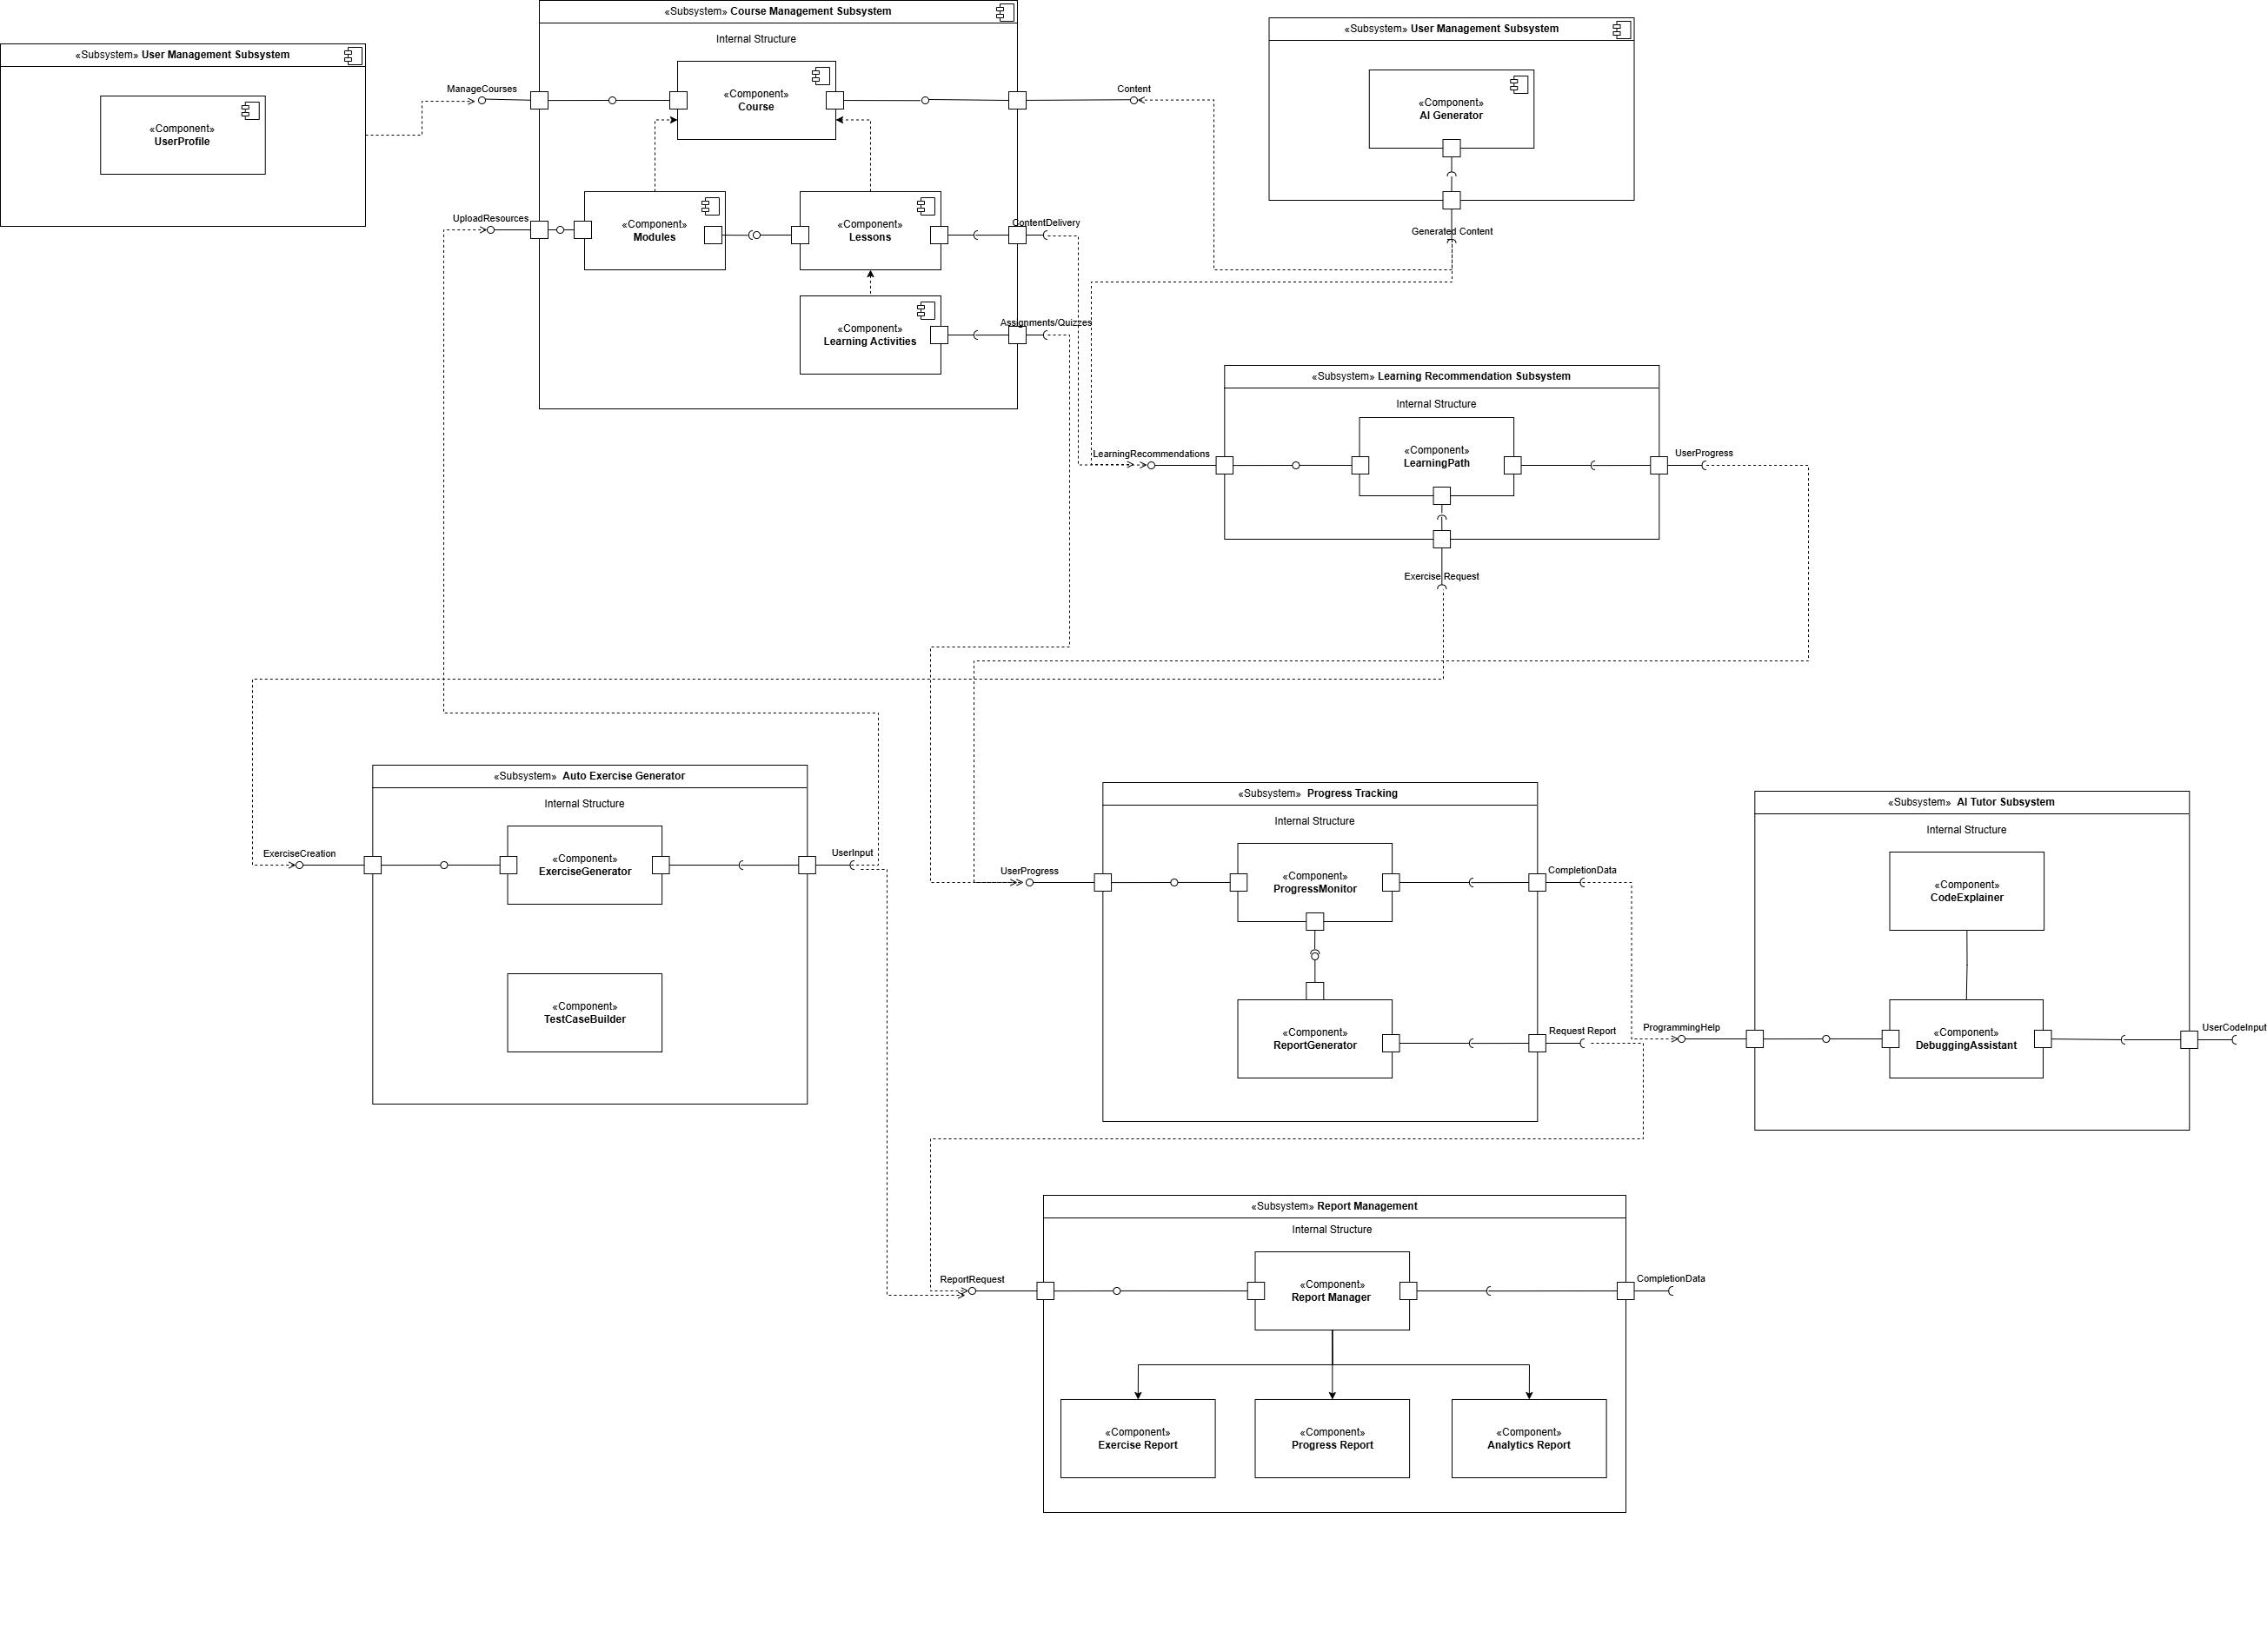
\includegraphics[width=\linewidth]{Images/component_diagram/component-All.drawio.png}
    \caption{Component-based Diagram cho toàn bộ hệ thống}
    \label{fig:enter-label}
\end{figure}
\begin{figure}[H]
    \centering
    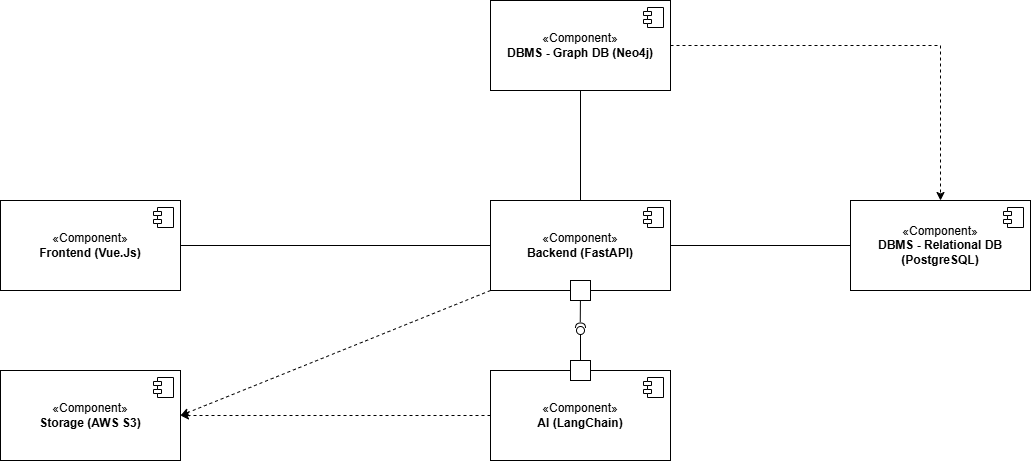
\includegraphics[width=\linewidth]{Images/component_diagram/component-Selected technologies.drawio.png}
    \caption{Component-based Diagram cho những công nghệ được chọn}
    \label{fig:enter-label}
\end{figure}
\newpage
\section{Database}
\subsection{EER diagram}
\begin{figure}[h!]
    \centering
    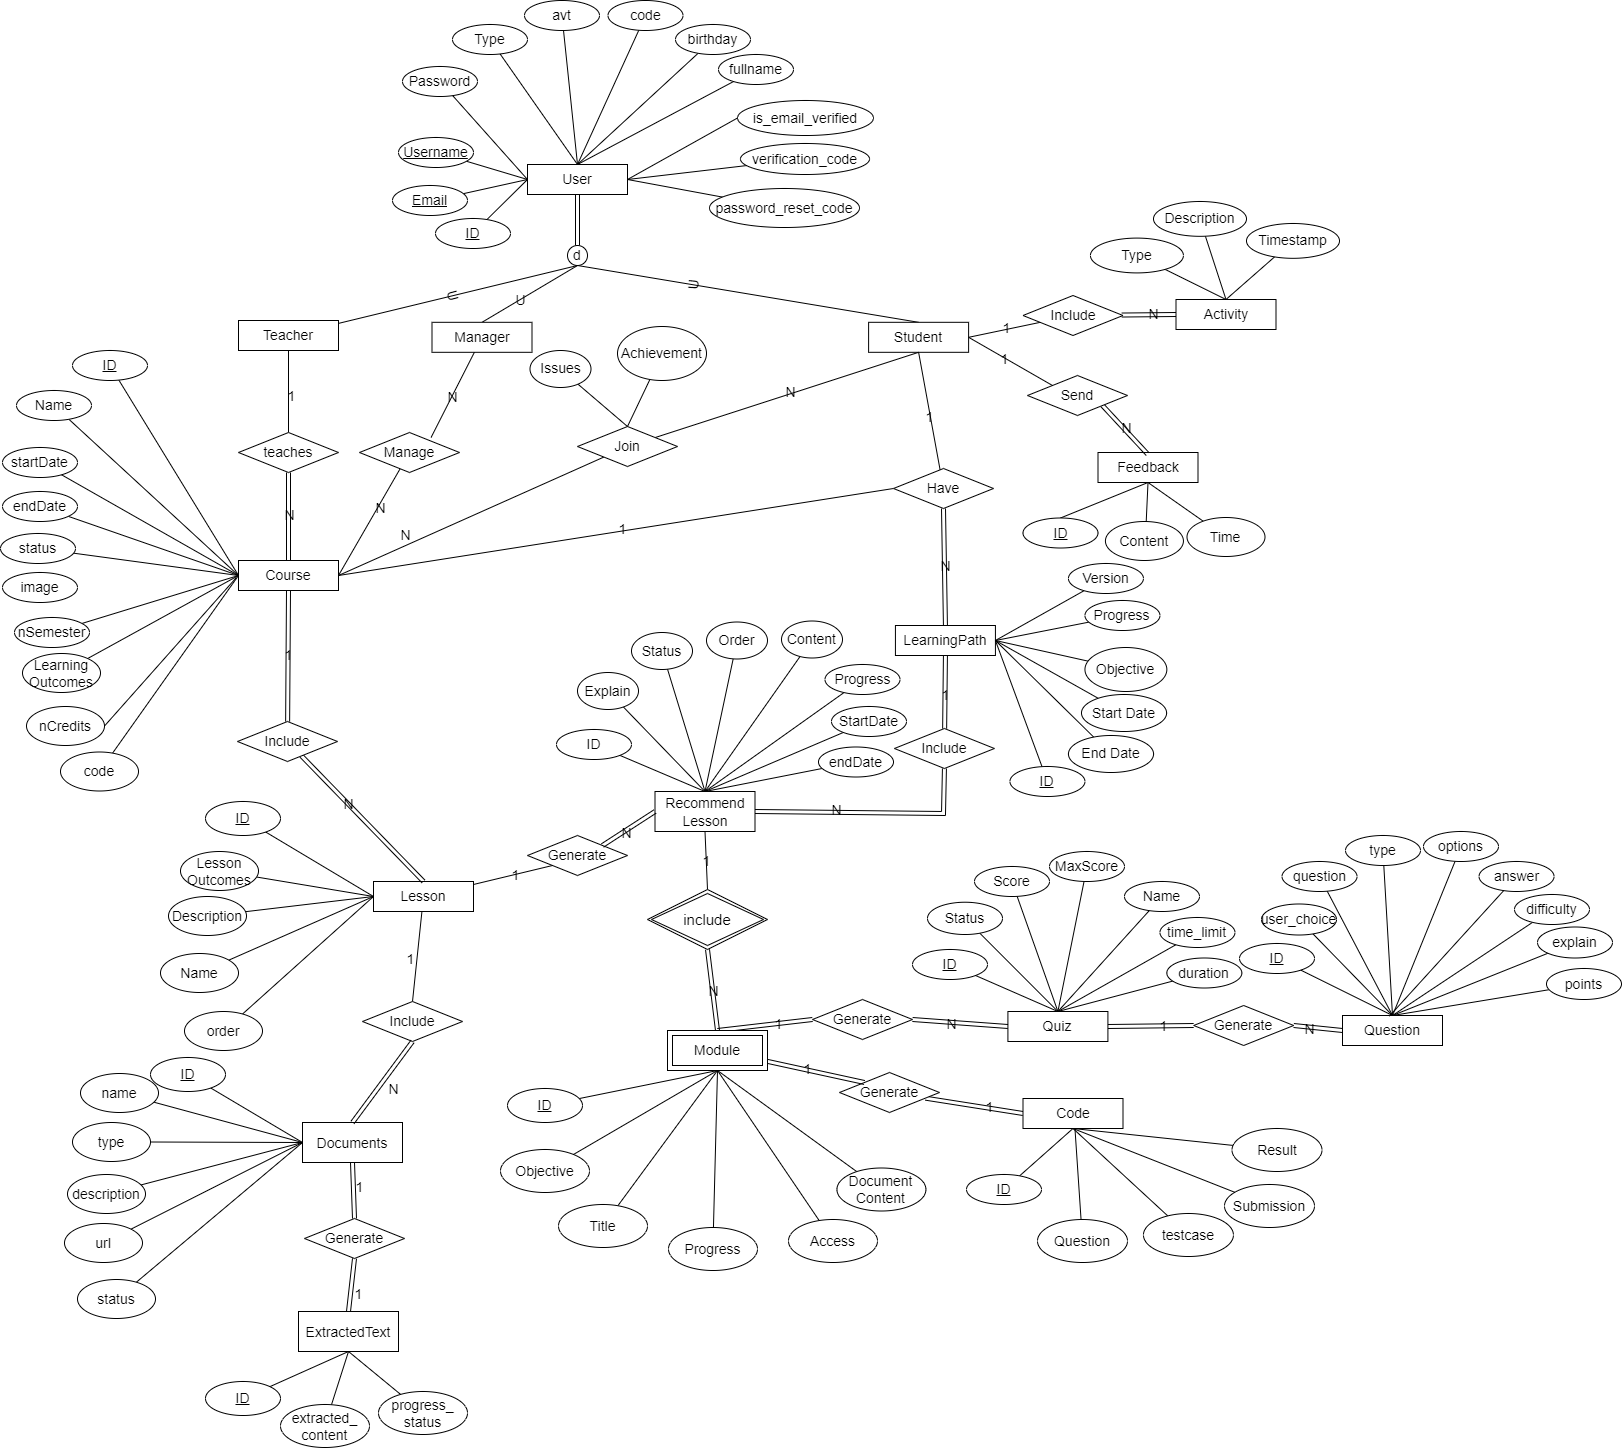
\includegraphics[width=\linewidth]{Images/Anh/EER.png}
    \caption{Sơ đồ EER của hệ thống}
    \label{fig:enter-label}
\end{figure}
\begin{enumerate}

    \item User có ba loại con: Teacher, Manager, và Student. Mỗi loại người dùng có các mối quan hệ khác nhau với các thực thể khác trong hệ thống:
    \begin{itemize}
        \item Student có các mối quan hệ sau:
        \begin{itemize}
            \item Include một hoặc nhiều Activity.
            \item Send nhiều Feedback cho hệ thống.
            \item Submit nhiều Exercise để thực hành.
            \item Join nhiều Course để tham gia các khóa học.
            \item Bookmark nhiều Lesson để lưu trữ các bài học quan trọng.
        \end{itemize}
        \item Teacher có thể Upload nhiều Course vào hệ thống để giảng dạy.
        \item Manager có thể Manage nhiều Course trong hệ thống, tức là có quyền quản lý các khóa học.
    \end{itemize}
    \item Course bao gồm nhiều Lesson, và mỗi khóa học có thể Include nhiều bài học khác nhau. Mỗi học viên (Student) có thể tham gia một khóa học và cho mỗi khóa học, họ sẽ có một LearningPath riêng biệt. Mối quan hệ này thể hiện rằng mỗi học viên có một lộ trình học tập cho mỗi khóa học mà họ tham gia.
    \item Lesson có thể Specialize thành Recommend Lesson, tức là các bài học có thể bao gồm các đề xuất học tập cho học viên. Mỗi bài học cũng có thể Include nhiều Module.
    \item LearningPath của mỗi học viên sẽ Have nhiều Recommend Lesson. Các lộ trình học tập này sẽ dẫn dắt học viên thông qua các bài học được đề xuất trong suốt quá trình học.
    \item Recommend Lesson có thể Include nhiều Module, tức là mỗi bài học được đề xuất có thể bao gồm nhiều mô-đun khác nhau để hỗ trợ học viên học tập một cách chi tiết hơn.
    \item Module có thể Generate nhiều Quiz để đánh giá kết quả học tập của học viên. Mỗi mô-đun cũng có thể Generate một tài liệu (Document) duy nhất liên quan đến nội dung học.
    \item Quiz chứa các câu hỏi và bài kiểm tra học viên, có thể bao gồm các phản hồi từ LLM Response, cung cấp thông tin về tên, độ khó, câu hỏi, câu trả lời, các lựa chọn, và hình ảnh liên quan đến bài kiểm tra.
    \item Document có thể được tạo ra từ các mô-đun và cũng có phản hồi từ LLM Response, giúp cung cấp thêm tài liệu học tập cho học viên.
    \item Activity bao gồm các hành động của người dùng trong hệ thống, và mỗi hoạt động có thể được Include bởi một hoặc nhiều User, đặc biệt là học viên.
    \item Feedback là thông tin phản hồi từ học viên gửi đến hệ thống và có thể được Send từ nhiều User, đặc biệt là từ học viên để cải thiện chất lượng giảng dạy và học tập.
\end{enumerate}
\newpage
\subsection{Lược đồ CSDL quan hệ ánh xạ}
\begin{figure}[h!]
    \centering
    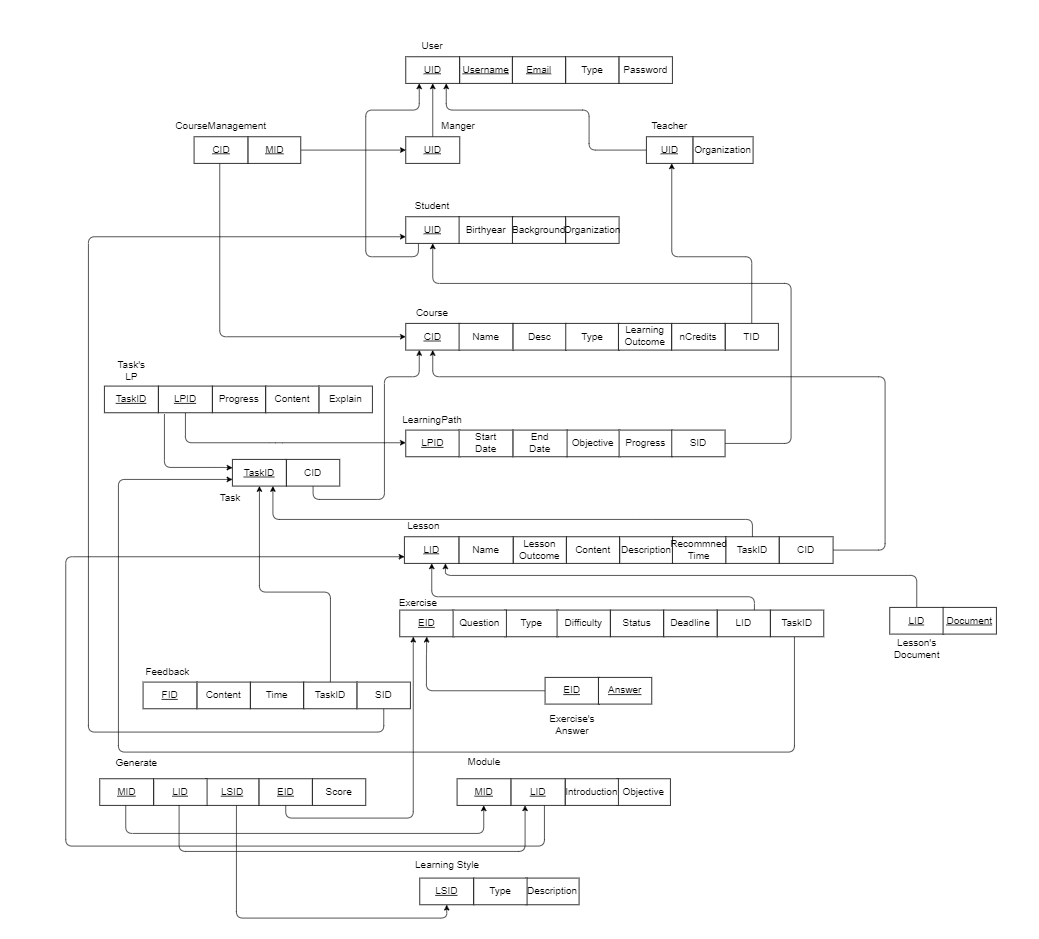
\includegraphics[width=\linewidth]{Images/Anh/mapping.png}
    \caption{Lược đồ CSDL quan hệ ánh xạ của hệ thống}
    \label{fig:enter-label}
\end{figure}
\newpage
\subsection{Class diagram}
\begin{figure}[h!]
    \centering
    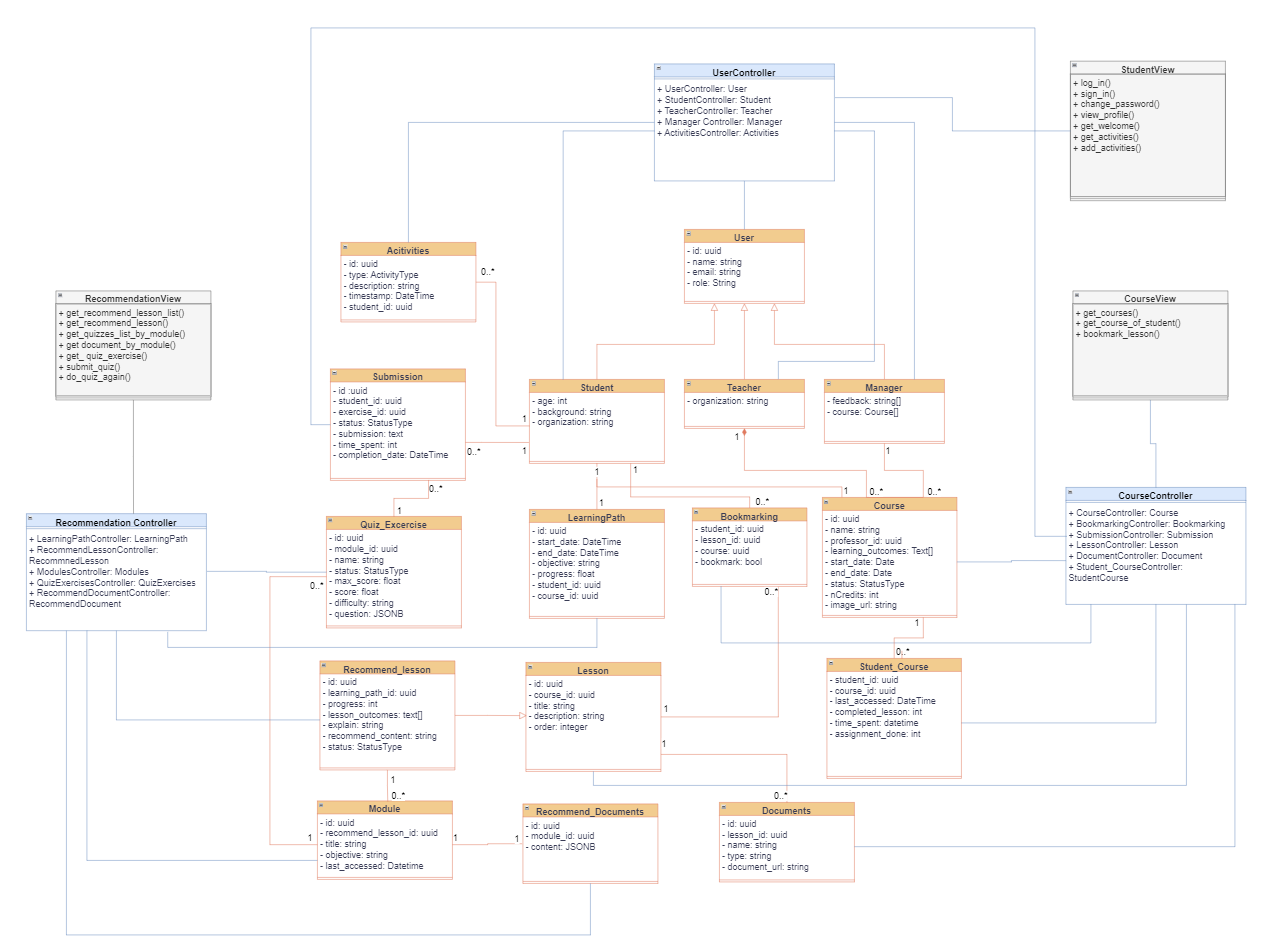
\includegraphics[width=\linewidth]{Images/Anh/classdiagram.png}
    \caption{Class diagram hiện thực của hệ thống}
    \label{fig:enter-label}
\end{figure}
Class diagram được thiết kế theo mô hình MVC mô tả một hệ thống học tập thông minh với ba vai trò chính là sinh viên, giáo viên và quản trị viên, tất cả đều kế thừa từ lớp người dùng (User). Mỗi người dùng có các chức năng cơ bản như đăng nhập, đăng xuất và cập nhật hồ sơ. Sinh viên chọn theo học khóa học của giảng viên, thực hiện bài tập, và theo dõi tiến độ học tập của mình. Lộ trình học tập bao gồm bài tập được cá nhân hóa cho từng sinh viên. Giáo viên chịu trách nhiệm tạo và quản lý các khóa học, bao gồm việc thêm bài tập, theo dõi kết quả học tập của sinh viên, và tạo ra các bộ câu hỏi kiểm tra. Quản trị viên có quyền quản lý toàn bộ hệ thống, bao gồm khóa học và người dùng, cũng như giải quyết các thắc mắc từ người dùng.
AI được sử dụng để hỗ trợ quá trình học tập thông qua việc tự động tạo lộ trình học tập và bài tập. AI dựa vào dữ liệu từ các tài liệu học tập, câu hỏi và đáp án có sẵn, cũng như các bài tập lập trình để cá nhân hóa trải nghiệm học cho người dùng.
\subsection{Sitemap}
\subsubsection{Sinh viên}
\begin{figure}[H]
    \centering
    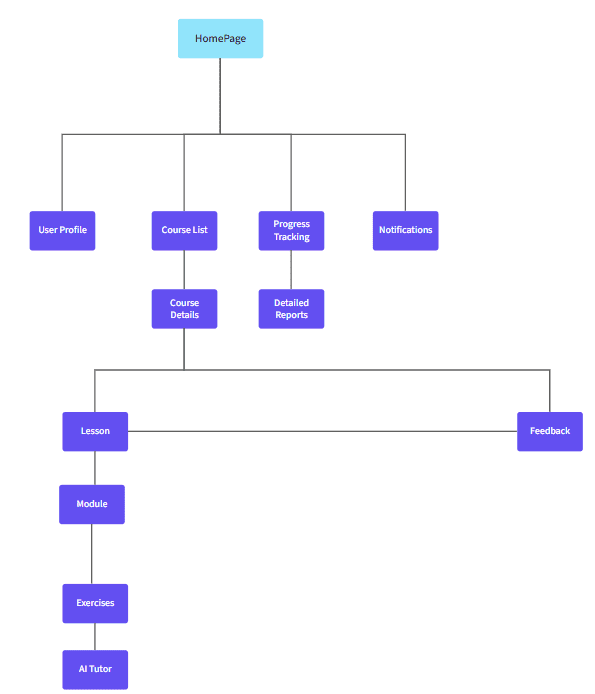
\includegraphics[scale=0.8]{Images/sitemap/Student.png}
    \caption{Sitemap cho đối tượng Sinh viên}
    \label{fig:enter-label}
\end{figure}
\par Sơ đồ trang web này thể hiện cấu trúc tổng thể của ứng dụng web, hiển thị các trang chính và mối quan hệ giữa chúng, đặc biệt là đối với đối tượng người dùng \textbf{Sinh viên}. Ở phía trên, có "Landing Page", "Log In Page" và "Dashboard Page". Đây là các trang điều hướng chính cho người dùng.
\par Bên dưới, có một số phần khác:

\begin{itemize}
    \item \textbf{User Profile:} Phần này chứa các trang liên quan đến tài khoản, thông tin cá nhân và cài đặt của sinh viên.
    \item \textbf{Course List Page:} Trang này hiển thị danh sách các khóa học mà sinh viên có thể truy cập.
    \item \textbf{Progress Tracking Page:} Trang này cho phép sinh viên theo dõi tiến độ và hiệu suất của họ trong các khóa học.
    \item \textbf{Notifications:} Phần này bao gồm trang chứa các thông báo cho sinh viên các cập nhật, tin nhắn hoặc cảnh báo quan trọng.
    \item \textbf{Course Detail Page:} Trang này cung cấp thông tin chi tiết về một khóa học cụ thể, như nội dung, mục tiêu và các tài nguyên khác.
    \item \textbf{Detailed Recommendation Lesson:} Trang này cung cấp các khóa học đề xuất học tập dựa trên tiến độ và mong muốn của người dùng.
    \item \textbf{Module Learning (Quiz), Module Learning (Code Exercises), and Module Learning (Reading Material):} Những phần này đại diện cho nội dung module của các bài học được đề xuất và chia thành 3 dạng bài tập như bài kiểm tra dạng quiz (multiple choices), bài tập lập trình thực hành và tài liệu đọc.
\end{itemize}
\par Nhìn chung, sơ đồ trang web này hiển thị các trang của hệ thống của đối tượng người dùng \textbf{Sinh viên} và cung cấp một cái nhìn tổng quan về cách các trang và chức năng liên quan được tổ chức và tương tác với nhau.
\subsubsection{Giảng viên}
\begin{figure}[H]
    \centering
    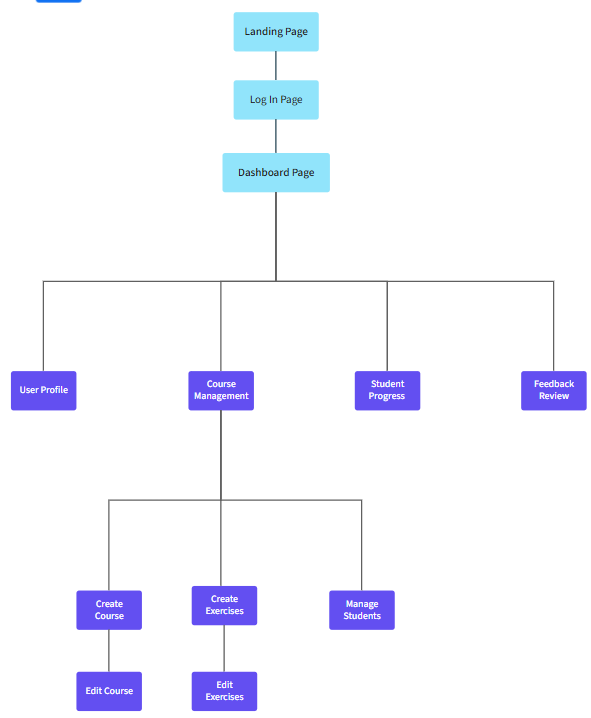
\includegraphics[scale=0.7]{Images/sitemap/Instructor.png}
    \caption{Sitemap cho đối tượng Giảng viên}
    \label{fig:enter-label}
\end{figure}
\par Sơ đồ trang web này đại diện cho cấu trúc của ứng dụng web, tập trung vào các chức năng và trang dành riêng cho giảng viên.

\par Ở phía trên, vẫn có các trang điều hướng chính như "Landing Page", "Log In Page" và "Dashboard Page", giúp giảng viên dễ dàng truy cập vào các phần quan trọng của hệ thống.

\par Bên dưới, sơ đồ được chia thành bốn phần chính:

\begin{itemize}
    \item \textbf{User Profile (Hồ sơ người dùng)}: Phần này chứa các trang liên quan đến thông tin cá nhân, tài khoản và cài đặt của giảng viên. Giảng viên có thể cập nhật thông tin cá nhân và quản lý các tùy chọn hệ thống của mình.
    \item \textbf{Course Management (Quản lý khóa học)}: Đây là phần quan trọng nhất với giảng viên, bao gồm các trang để tạo, chỉnh sửa, và quản lý các khóa học mà họ giảng dạy. Giảng viên có thể thêm các bài giảng, tài liệu học, và bài kiểm tra cho sinh viên.
    \item \textbf{Student Progress (Tiến độ học sinh)}: Phần này giúp giảng viên theo dõi và giám sát tiến độ học tập của sinh viên trong các khóa học mà họ giảng dạy. Giảng viên có thể xem thông tin về kết quả học tập của sinh viên, bao gồm điểm kiểm tra, bài tập và các hoạt động học tập khác.
    \item \textbf{Feedback Management (Quản lý phản hồi)}: Phần này cho phép giảng viên thu thập, quản lý và phân tích phản hồi từ sinh viên về khóa học, bài giảng, hoặc các hoạt động học tập. Đây là công cụ hữu ích để giảng viên đánh giá mức độ hiệu quả của phương pháp giảng dạy và cải thiện chất lượng khóa học.
\end{itemize}

\par Các trang con trong mỗi phần cung cấp các chức năng cụ thể hơn, chẳng hạn như chỉnh sửa nội dung khóa học, xem bảng điểm và thông tin phản hồi từ sinh viên.

\par \textbf{Tổng quan:} Sơ đồ trang web này cung cấp cái nhìn tổng quát về các chức năng chính mà giảng viên cần để quản lý khóa học, theo dõi tiến độ sinh viên và thu thập phản hồi. Cấu trúc đơn giản, dễ sử dụng, giúp giảng viên dễ dàng thực hiện các công việc quản lý và giảng dạy hiệu quả.
\subsubsection{Manager}
\begin{figure}[H]
    \centering
    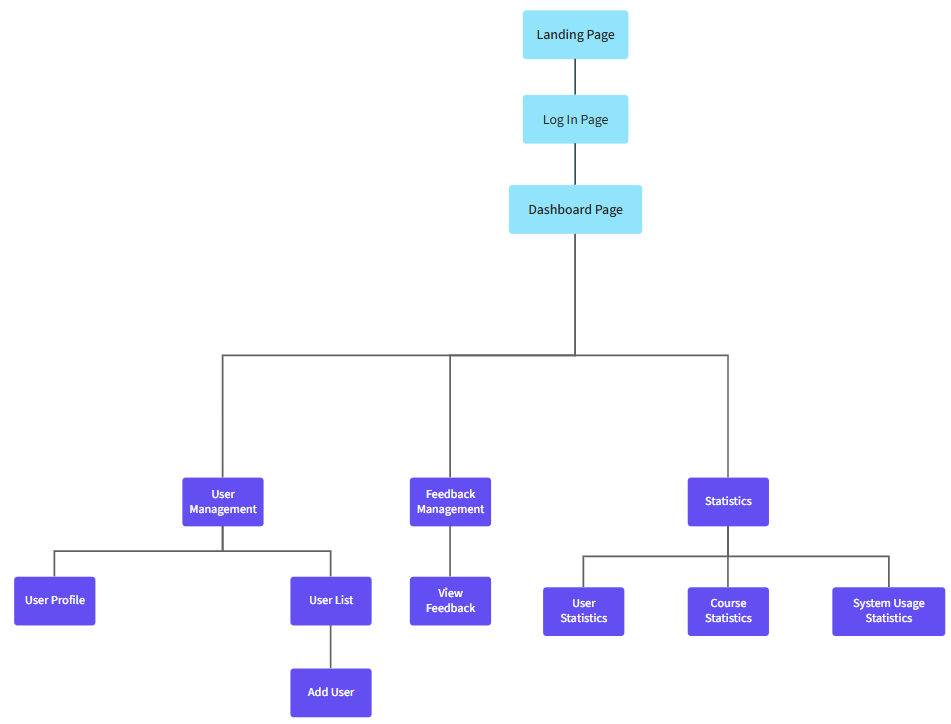
\includegraphics[scale=0.55]{Images/sitemap/Manager.png}
    \caption{Sitemap cho đối tượng Quản trị viên}
    \label{fig:enter-label}
\end{figure}
\par Sơ đồ trang web này cung cấp cái nhìn tổng quát về các chức năng chính mà Admin cần để quản lý các chức năng người dùng.

\par Ở phía trên, các trang điều hướng chính vẫn là "Landing Page", "Log In Page", và "Dashboard Page".

\par Các phần chính trong sơ đồ trang web này là:

\begin{itemize}
    \item \textbf{User Management:} Phần này bao gồm các trang để quản lý hồ sơ cá nhân, cài đặt và thông tin tài khoản của người dùng.
    \item \textbf{Feedback Management:} Phần này tập trung vào các trang để cung cấp phản hồi, đánh giá và nhận xét liên quan đến trải nghiệm học tập của người dùng.
    \item \textbf{Statistics:} Phần này cung cấp các trang hiển thị các số liệu thống kê, chỉ số và dữ liệu liên quan đến tiến độ, hiệu suất và mức độ sử dụng hệ thống của người dùng.
\end{itemize}

\par Các trang cấp thấp hơn trong sơ đồ trang web này hướng đến học sinh, chẳng hạn như các trang để xem chi tiết khóa học, truy cập tài liệu học tập và theo dõi tiến độ cá nhân.

\par Sơ đồ trang web này gợi ý về một ứng dụng web được thiết kế để cung cấp cho học sinh một trải nghiệm học tập cá nhân hóa, với sự tập trung vào quản lý người dùng, phản hồi và các thông tin chi tiết dựa trên dữ liệu để hỗ trợ hành trình giáo dục của họ.
\section*{Tổng kết}

Nhìn chung, ba sơ đồ trang web này thể hiện các góc nhìn và ưu tiên khác nhau trong thiết kế và chức năng của ứng dụng web, đáp ứng nhu cầu của các loại người dùng khác nhau, chẳng hạn như học sinh, giảng viên và quản trị viên.